\section{Разработка и обоснование варианта схемы параллелизма алгоритма}\label{sec:devAlgoParallel}
\begin{figure}[h]
    \begin{center}
        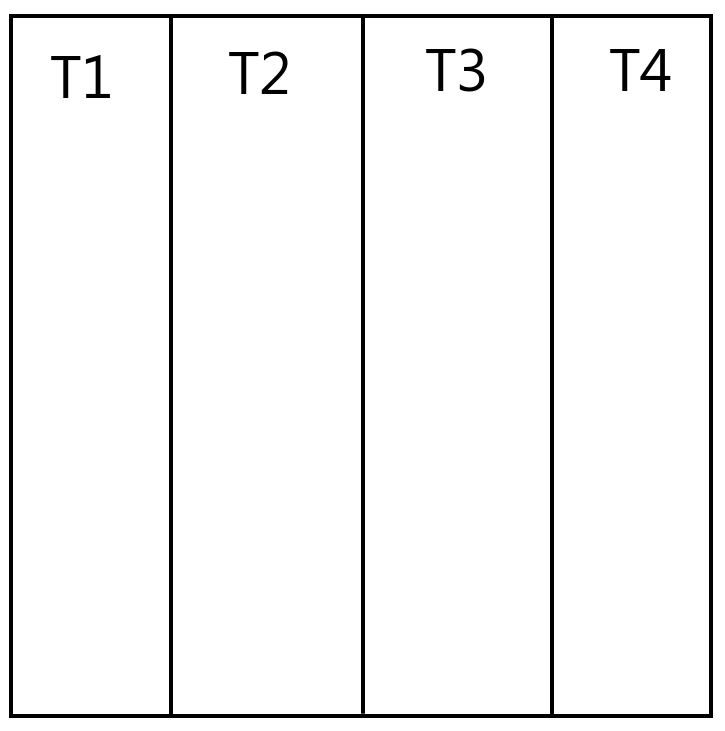
\includegraphics[width=0.5\textwidth]{../resources/img}
    \end{center}
    \caption{Схема разделения изображения между потоками выполнения.}
    \label{fig:imageThreads}
\end{figure}

Как показано на рисунке~\ref{fig:imageThreads} изображение делится между потоками очень несложно.
Всего есть 4 потока: T1, T2, T3, T4.
Каждый поток выполнения получает в своё распоряжение четверть исходной картинки.
Причём она делится не на квадраты, а на полосы, так как при таком подходе сильно упрощается кодирование и появляется возможность добавить сколь угодно много потоков.
При этом не возникает гонок процессов на ресурсы.
Каждый процесс работает только в отведенной ему области основной и буферной матрицы.
Проблемы могут появиться только на стыке областей ответственности двух процессов, но даже это невозможно, так ка используется буферная матрица.
Поэтому изображение будет точно так же, как при использовании однопоточной системы.

Для реализации многопоточности, необходимо изменить функции обработки изображения таким образом, чтобы они могли работать с частью матрицы.
Реализуется это очень просто, нужно добавить аргумент начала и конца текущего блока обработки и передать их в корневой \texttt{for}.
Так как в \textbf{bitmap} первый параметр --- x, а второй --- y, то разделение получается вертикальное.

Не менее важно вовремя синхронизовать потоки выполнения.
Если этого не сделать, то на финальном изображении могут появиться артефакты на стыках работы двух потоков.
Поэтому, перед выполнением уменьшения и увеличения потоки должны синхронизоваться.

